\subsection{Utledning av bølgeligningen}
\subsubsection{Forhåndsbetingelser}
For å finne frem til bølgeligningen må man analysere systemet som likningen skal brukes på.
På en gitarstreng er lengden justerbar, men tonen endres primært ved å stramme eller slakke
strengen.

En gitarstreng modelleres som en tråd som er spent mellom to punkter, der den er fiksert på plass.
I normaltilstand ligger strengen stram i en rett linje mellom punktene, frem til den plukkes. Da
forstyrres likevekten, og strengen begynner å vibrere. Problemet er da å finne en $u(x,t)$ som modellerer
defleksjonen til strengen. Hvis strengen har lengde $l$, massetetthet $\rho$ og slippes ved $t=0$,
vil modellen beskrive defleksjonen $u(x,t)$ for vilkårlig $x$ når $t>0$.

Forutsetninger for løsning av bølgeligningen:

\begin{enumerate}
  \item Gravitasjon er neglisjerbar i forhold til strengspenningen.
  \item Alle defleksjoner er små og skjer i samme plan.
  \item Massen per lengde er konstant over hele strengen, slik at spenningen er den samme
  gjennom hele strengen.
\end{enumerate}
\clearpage
\subsubsection{Utledning}

\begin{figure}[H]
  \centering
  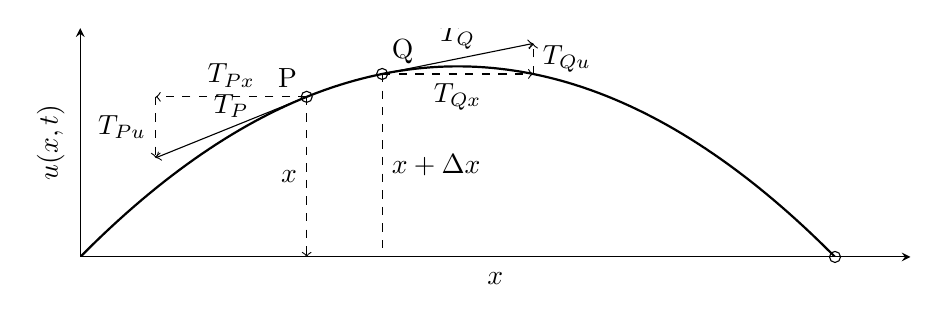
\begin{tikzpicture}
    \begin{axis}[
      width=\textwidth,
      height=0.37\textwidth,
      axis lines=left,
      xlabel={$x$},
      ylabel={$u(x,t)$},
      xmin=0, xmax=1.1,
      ymin=0, ymax=0.6,
      xtick=\empty,
      ytick=\empty
    ]

      % punkter
      \coordinate (Ppoint)  at (axis cs:0.3,0.42);
      \coordinate (Pupoint) at (axis cs:0.1,0.26);
      \coordinate (Pxpoint) at (axis cs:0.1,0.42);
      \coordinate (Qpoint)  at (axis cs:0.4,0.48);
      \coordinate (Qupoint) at (axis cs:0.6,0.56);
      \coordinate (Qxpoint) at (axis cs:0.6,0.48);

      % strengkurve
      \addplot[domain=0:1, samples=100, thick] {-2*x^2 + 2*x};

      % krefter ved P
      \draw[->, thin] (Ppoint) -- (Pupoint) node[midway, above] {$T_P$};
      \draw[->, thin, dashed] (Ppoint) -- (Pxpoint) node[midway, above] {$T_{Px}$};
      \draw[->, thin, dashed] (Pxpoint) -- (Pupoint) node[midway, left]  {$T_{Pu}$};

      % krefter ved Q
      \draw[->, thin] (Qpoint) -- (Qupoint) node[midway, above] {$T_Q$};
      \draw[->, thin, dashed] (Qpoint) -- (Qxpoint) node[midway, below] {$T_{Qx}$};
      \draw[->, thin, dashed] (Qxpoint) -- (Qupoint) node[midway, right] {$T_{Qu}$};

      % loddrette hjelpelinjer
      \draw[->, dashed] (axis cs:0.3,0.42) -- (axis cs:0.3,0) node[midway, left] {$x$};
      \draw[dashed]     (axis cs:0.4,0.48) -- (axis cs:0.4,0) node[midway, right] {$x+\Delta x$};

      % punktsymboler og etiketter
      \addplot[only marks, mark=o] coordinates {(0.3,0.42) (0.4,0.48) (1,0)};
      \node[anchor=south east] at (Ppoint) {P};
      \node[anchor=south west] at (Qpoint) {Q};
      \node[anchor=north]      at (axis cs:1,0) {$l$};

    \end{axis}
    \end{tikzpicture}
  \caption{Krefter og vinkler på et lite strengstykke $[x,\,x+\Delta x]$.}
\end{figure}

For å finne likningen betraktes et lite stykke av strengen ved $t=0$, med lengde $\Delta x$ og start i
$x$. Punktet $P=(x,u(x,0))$ og punktet $Q=(x+\Delta x, u(x+\Delta x,0))$ er endene av strengstykket.
$T$ er kraften som spenningen i strengen skaper i et punkt $x>0$ langs strengen. 
$\alpha$ er vinkelen mellom $T_{Qx}$ og $T_Q$, og $\beta$ er vinkelen mellom
$T_{Px}$ og $T_P$.

\begin{align*}
  T_{Px} = T_P \cos\beta, &\qquad T_{Qx} = T_Q \cos\alpha,\\
  T_{Pu} = T_P \sin\beta, &\qquad T_{Qu} = T_Q \sin\alpha.
\end{align*}

Fordi spenningen i strengen er lik over hele strengen, vil de horisontale kreftene
av $T_Q$ og $T_P$ utjevne hverandre:

\begin{equation}
  T_{Px} = T_{Qx} = T = \text{const.}
  \label{eq:horisontaleKrefterKonstant}
\end{equation}

Ifølge Newtons andre lov $(F=ma)$ for strengstykket settes massen lik $m=\rho\,\Delta x$ og
akselerasjonen $a=u_{tt}$. Kraften som virker på strengen er $F=T_{Qu}-T_{Pu}$. Da får vi:

\begin{equation*}
  T_{Qu}-T_{Pu}=\rho\,\Delta x\,\frac{\partial^2 u}{\partial t^2}.
\end{equation*}

Videre brukes $\tan\theta=\frac{\sin\theta}{\cos\theta}$ sammen med \eqref{eq:horisontaleKrefterKonstant}, og
$\tan\alpha$ og $\tan\beta$ antas små (små defleksjoner), slik at forenklinger kan benyttes: 

\begin{equation}
  \frac{T_{Qu}}{T_{Qx}}-\frac{T_{Pu}}{T_{Px}}
  = \tan\alpha - \tan\beta
  = \frac{\partial u}{\partial x}(x+\Delta x,t)-\frac{\partial u}{\partial x}(x,t)
  = \frac{\rho\,\Delta x}{T}\,\frac{\partial^2 u}{\partial t^2}.
  \label{eq:krefterPaStykke}
\end{equation}
\clearpage
Ganger man begge sider med $\dfrac{T}{\rho\,\Delta x}$:

\begin{equation}
  \frac{\partial^2 u}{\partial t^2}
  = \frac{T}{\rho\,\Delta x}\left[
     \frac{\partial u}{\partial x}(x+\Delta x,t)-\frac{\partial u}{\partial x}(x,t)
    \right].
  \label{eq:tidPartiellDerivert}
\end{equation}

Setter man $\Delta x\to 0$ som grenseverdi, fremkommer definisjonen av den deriverte:

\begin{equation}
  \frac{\partial^2 u}{\partial t^2}
  = \lim_{\Delta x\to 0}\frac{T}{\rho}\frac{1}{\Delta x}
    \left[\frac{\partial u}{\partial x}(x+\Delta x,t)-\frac{\partial u}{\partial x}(x,t)\right]
  = \frac{T}{\rho}\,\frac{\partial^2 u}{\partial x^2}.
  \label{eq:deltaXGarMotNull}
\end{equation}

Setter man $c^2=\dfrac{T}{\rho}$ får vi bølgeligningen: 

\begin{equation}
  \frac{\partial^2 u}{\partial t^2}
  = c^2\,\frac{\partial^2 u}{\partial x^2},
  \qquad
  c^2=\frac{T}{\rho}.
  \label{eq:utledetBolgelikning}
\end{equation}

\subsection{Metode og verktøy for numerisk løsning}
\subsubsection{Valg av verktøy}
For å løse bølgeligningen numerisk har vi valgt å bruke Python. Språket er mye brukt innen
vitenskapelige beregninger og har et stort økosystem av biblioteker som forenkler implementasjon av
numeriske metoder og visualisering av resultater. Innenfor bibliotekene \texttt{NumPy} og \texttt{Matplotlib}
finnes funksjonalitet som gjør det enkelt å løse oppgaver numerisk og fremstille resultatene grafisk.
Dette gjør Python til et velegnet valg for denne problemstillingen. For animasjoner av resultatene bruker
vi \texttt{matplotlib.animation} (en del av \texttt{Matplotlib}); dette gir en mer intuitiv forståelse av
hvordan løsningen utvikler seg over tid. Til 2D-grafer benyttes \texttt{matplotlib.pyplot}. For å forstå
komplekse ligninger som bølgeligningen er det nyttig å kunne visualisere resultatene på en enkel og
konsis måte.

\subsection{Løsning med separasjon av variable}
\begin{equation}
	u_{tt} = c^2 u_{xx} \qquad \iff \qquad 
	\frac{\partial^2 u}{\partial t^2} = \frac{T}{\rho} \frac{\partial^2 u}{\partial x^2}	
	\label{eq:bølgelikningForLøsning}
\end{equation}

En løsning av bølgeligningen forutsetter definerte rand- og initialbetingelser. Strengen har fast lengde $l$
og er festet i begge ender; dette er randbetingelsene. Initialbetingelsene gjelder ved $t=0$, hvor strengen
slippes fra en posisjon bestemt av $f(x)$. Ettersom strengen slippes, settes $u_t(x,0) = 0$.
\clearpage
Grensebetingelsene for funksjonen $u(x,t)$ blir derfor:

\begin{align}
	u(0 , t) = 0 \label{eq:grensebetingelse0}\\
	u(l , t) = 0 \label{eq:grensebetingelsel}
\end{align}

og initialbetingelsene for funksjonen $u(x,t)$ blir:

\begin{align}
	u(x , 0) &= f(x) = \sum_{n=0}^{n=\infty} c_n \sin \left( \frac{n \pi}{l} x \right) 	
	\label{eq:initialbetingelse1}
\end{align}

Separasjon av variabler går ut på å finne to funksjoner $F(x)$ og $G(t)$ slik at $u(x , t)=F(x)G(t)$.
Da separeres tid $t$ og posisjon $x$ i to ulike funksjoner.

\begin{equation*}
	u(x , t) = F(x)G(t)
\end{equation*}

De partiellderiverte av $F(x)$ og $G(t)$ blir:

\begin{equation}
	u_{tt} = F(x)G''(t), \qquad u_{xx} = F''(x)G(x)
	\label{eq:separasjonPartiellDeriverte}	
\end{equation}

Setter vi \eqref{eq:separasjonPartiellDeriverte} inn i \eqref{eq:bølgelikningForLøsning}:

\begin{align*}
  \hspace{35ex}
  u_{tt} &= c^2 u_{xx} \\
  \hspace{2ex} F(x)G''(t) &= c^2 F''(x)G(t) \hspace{10ex} \vert 
  \cdot \frac{1}{c^2 F''(x) G''(t)} \\
  \frac{F''(x)}{F(x)} &= \frac{1}{c^2} \frac{G''(t)}{G(t)}
\end{align*}

For at begge sider skal være like for alle $x \in \left[ 0 , l \right]$ og $t < 0$ må uttrykket være lik en
konstant. Denne settes til $- \lambda^2$. Den velges negativ for å gi sinus- og cosinusløsninger (ikke
eksponentielle). Med kvadrert parameter sikres positivitet:

\begin{equation*}
	\frac{F''(x)}{F(x)} = \frac{1}{C^2} \frac{G''(t)}{G(t)} = - \lambda^2
\end{equation*}
\clearpage
$F(x)$ og $G(t)$ er dermed to differensiallikninger som kan løses. Med $F(x)$, og
grensebetingelsene (\ref{eq:grensebetingelse0}) og (\ref{eq:grensebetingelsel}) blir første differensialligning mulig å løse:

\begin{align*}
	\hspace{20ex} \frac{F''(x)}{F(x)} &= - \lambda^2 \hspace{10ex} \vert \cdot F(x)\\
	F''(x) + \lambda^2&F(x) = 0
\end{align*}

Løses dette som en 2.\ ordens homogen differensiallikning blir resultatet:

\begin{align*}
	F''(x) + \lambda^2&F(x) = 0 \\ 
	\Rightarrow r^2 + &\lambda^2 = 0 \\
	\Rightarrow r_1 = 0 - i \lambda &\vee r_2 = 0 + i \lambda \\
	\Rightarrow F(x) = e^{0 \cdot x} & \left( \alpha  \cos \lambda x + \beta \sin \lambda x \right) \\
	\Rightarrow F(x) = \alpha \cos& \lambda x + \beta \sin \lambda x 
\end{align*}

Settes grensebetingelse (\ref{eq:grensebetingelse0}) inn:

\begin{align*}
	u(0 , t) = F(&0)G(t) = 0\\
	\Rightarrow F(0) = \alpha \cos&\lambda \cdot 0 + \beta \sin \lambda \cdot 0 \\
	\Rightarrow F(0) = \alpha \cos&0 + \beta \sin 0 \\
	\Rightarrow F(0) = &\alpha = 0 \\
	\Rightarrow \alpha =& 0 \\
	\Rightarrow F(x) = &\beta \sin \lambda x
\end{align*}

Videre brukes grensebetingelse (\ref{eq:grensebetingelsel}) for å finne $\lambda$:

\begin{align*}
	u(l ,t) = F(l&)G(t) = 0 \\
	\Rightarrow F(l) =& 0 \\
	\Rightarrow \beta \sin \lambda &\cdot l = 0 \\ 
	\Rightarrow \lambda = \frac{\pi n}{l}&, \qquad n \in \mathbb{N} \\
	\Rightarrow F(x) = { \beta }_n & \sin \frac{\pi n}{l} x
\end{align*}

Nå er uttrykket for $\lambda$ og $F(x)$ funnet; neste steg er å finne $G(t)$:

\begin{align*}
	G''(t) = - \lambda^2 & c^2 G(t) \\
	\Rightarrow G''(t) + \lambda^2 & c^2 G(t) = 0 
\end{align*}

Dette løses som en 2.\ ordens homogen differensiallikning:

\begin{align*}
	G''(t) + \lambda^2 & c^2 G(t) = 0 \\
	\Rightarrow r^2 + \lambda^2 c^2 = 0 \\
	\Rightarrow r_1 = 0 + i \lambda c &\vee r_2 = 0 - i \lambda c \\ 
	\Rightarrow G(t) = e^{0 t} \gamma&\cos c \lambda t + \psi \sin c \lambda t \\
	\Rightarrow G(t) = \gamma\cos & c \lambda t + \psi \sin c \lambda t
\end{align*}

Ettersom strengen slippes fra startposisjonen bestemt av (\ref{eq:initialbetingelse1}) og startfarten settes til $u_t(x,0)=0$,
blir $\psi=0$, og $G(t)$ reduseres til:

\begin{equation*}
	G(t) = \gamma \cos c \lambda t = \gamma \cos \frac{c \pi n}{l} t
\end{equation*}

Settes sammen $F(x)$ og $G(t)$, blir løsningen:

\begin{equation}
	u(x,t) = \sum_{n=0}^{\infty} c_n 
	\sin \left( \frac{n \pi}{l} x \right)
	\cos \left( \frac{n \pi c}{l} t \right)
	\label{eq:bølgelikningLøst}	
\end{equation}

\subsubsection{Konstanten \texorpdfstring{$c_n$}{cn}}

Konstanten $c_n$ beskriver initialbetingelsene. For en streng med lengde
$l$ og initialform $f(x)$ (slik at $u(x,0)=f(x)$) blir:

\begin{equation}
	c_n = \frac{2}{l} \int_{0}^{l} f(x) \sin \left( \frac{n \pi}{l} x \right) \,dx
	\label{eq:cnDefinisjon}
\end{equation}

\subsubsection{Beskrivelse av maple kode}

Maple-koden starter med å definere initialbetingelsene for simuleringen. Strengen er $l = 64{,}77\,\text{cm}$ lang og dras
opp i punkt $x = a = 7\,\text{cm}$ til høyde $u(a,0) = h = 2\,\text{cm}$. For å estimere tettheten til gitarstrenger brukes 
formelen $\rho = 7825\,\text{kg/m}^3 \cdot \pi (0.00256 \cdot \texttt{string\_gauge} /2)^2$. Strengtykkelsene er hentet fra
Ernie Ball Super Slinky \parencite{ErnieBallSlinky}, og $7825\,\text{kg/m}^3$ er massetetthet for stål ifølge Wikipedia \parencite{WikipediaTetthet},
idet det antas at alle strengene er stålstrenger. Ved beregning av strengspenning ble en strengspenningskalkulator brukt
\parencite{RodrigoStringTensionCalc}, med valg «0.009 D'Addario / Ernie Ball». Deretter defineres $f(x)$, $c_n$ og $u(x,t)$,
og \verb|explore| samt \verb|plot| benyttes for å visualisere alle strengene i én graf, der $t$ styres med en glider.
Det var ikke trivielt å legge inn strengenes navn i plottet, noe som gjør det vanskelig å skille kurvene. Under følger en tabell
med strengtykkelser, massetetthet, strengspenning og $c$-verdi. Koden fra maple kan hentes her: \parencite{mapleKode}

\begin{table}[!h]
	\centering
	\begin{tabular}{|c|c|c|c|c|}
		\hline
		Streng & strengtykkelse & massetetthet, $\rho$ & strengspenning, $T$ & $c$-verdienre \\  
		\hline
		E4 & $0.009''$ & $3,26 mg/m$ & $58,49N$ & $4,24 km/s$ \\	
		B3 & $0.011''$ & $4,87 mg/m$ & $47.99N$ & $3,14 km/s$ \\
		G3 & $0.016''$ & $10,3 mg/m$ & $65,29N$ & $2,51 km/s$ \\
		D3 & $0.024''$ & $23,2 mg/m$ & $69,62N$ & $1,61 km/s$ \\
		A2 & $0.032''$ & $41,2 mg/m$ & $70,09N$ & $1,30 km/s$ \\
		E2 & $0.042''$ & $71,0 mg/m$ & $65,06N$ & $1,16 km/s$ \\
		\hline
	\end{tabular}
	\caption{Tabell over gitarstrenger og deres respektive fysiske verdier}
	\label{tab:listeOverGitarstrenger}
\end{table}

\subsection{Beskrivelse av kode for numerisk løsning}
\subsubsection{Pakker, variabler og parametere}
I dette delkapittelet beskrives en numerisk tilnærming til bølgeligningen (koden kan hentes fra 
\parencite{simuleringKode}). 

Først importeres nødvendige pakker for numeriske beregninger og grafisk fremstilling: \texttt{NumPy} for numerikk,
\texttt{matplotlib.pyplot} for plotting og \texttt{matplotlib.animation} for animasjon (jf.\ forrige seksjon).
Deretter settes konfigurasjonsparametere som definerer strengens fysiske egenskaper og parametere for den numeriske 
løsningen. Dette inkluderer lengden $L$, bølgehastigheten $c$ og simulert varighet $s$. Videre defineres antall
punkter $N$ til å dele opp strengen. Dette påvirker nøyaktigheten: flere punkter gir bedre oppløsning, men øker
beregningstid og minnebruk. Antall moduser bestemmer detaljgraden i startformen, der høyere verdi gir skarpere kanter og
mer høyfrekvent innhold. 

Videre settes grafiske parametere, som \texttt{fps} (frames per second) for animasjonen og linjetykkelse. Startformen 
settes med
\begin{lstlisting}
  initial_shape_type = "pluck"
  pluck_width: float = 0.15
\end{lstlisting}
der \verb|"pluck"| angir en plukk (trekant-/teltform), og \verb|pluck_width| definerer bredden på området som plukkes.

\subsubsection{Initialbetingelser-funksjonen}
Hensikten er å definere startformen ved $t=0$, altså å returnere $u(x,0)$.
Funksjonen tar inn en $\verb|x|$-array (posisjoner langs strengen). Avhengig av \verb|initial_shape_type|
returneres ulike startformer. I vårt tilfelle gir \verb|"pluck"| en trekantformet profil, der plukkposisjon og bredde styrer formen:
\begin{lstlisting}
  if initial_shape_type == "pluck":
    center = pluck_position * length_m
    width = pluck_width * length_m
    return np.clip(1.0 - np.abs(x - center) / width, 0.0, 1.0)
\end{lstlisting}

Med verdiene satt i starten av koden får vi figuren under:

\begin{figure}[H]
    \centering
    \begin{tikzpicture}
        \begin{axis}[
        width=0.9\textwidth,
        height=0.5\textwidth,
        axis lines=left,
        xlabel={$x$ [m]},
        ylabel={$u(x,0)$ [m]},
        xmin=0, xmax=1.02,
        ymin=-1.1, ymax=1.1,
        xtick={0.15, 0.45, 1},
        ytick={-1, 0, 1}
        ]
        
        \draw (0,0) -- (0.15,0);
        \draw [dashed] (0.15,0) -- (0.3,1) -- (0.45,0);
        \draw (0.45,0) -- (1,0);
        \fill (0.3,1) circle (2pt);

        \end{axis}
    \end{tikzpicture}
    \caption{Startform ved $t=0$ når strengen plukkes ved $x=0.3$ m.}
\end{figure}

Her ser vi at strengen plukkes i en trekantformet bølge med høyde $y=1.0\,\text{m}$ og bredde $0.15\,\text{m}$.
Dette er ikke en nøyaktig kopi av en fysisk plukk, men en hensiktsmessig tilnærming som er enkel å implementere.

Startfarten settes til null over hele strengen ved $t=0$. Funksjonen $g(x)=u_t(x,0)$ returnerer derfor
\verb|np.zeros_like(x)| (en array med samme form som \verb|x|, men med bare nuller).

\subsubsection{Oppsett av romlige og tidsmessige akser}
Første linje (\verb|np.ndarray x|) oppretter et jevnt fordelt rutenett fra $0$ til lengden $L$. Punktene representerer
posisjoner der $u(x,t)$ evalueres. Som eksempel: med \verb|num_points=5| og \verb|length_m=1.0| blir \verb|x = [0, 0.25, 0.5, 0.75, 1.0]|.
Variabelen \verb|dx| beregnes for informasjon (ikke brukt videre). Deretter settes tidssteget \verb|dt| til $\tfrac{1}{\texttt{fps}}$,
slik at for \verb|fps=60| oppdateres tilstanden hver $\approx 16{,}7$ ms. Antall tidssteg settes med
\verb|num_steps = int(duration_s * fps) + 1|, og \verb|t| blir arrayen med alle tidspunkter der strengen evalueres.

\subsubsection{Metodefunksjonen}
Denne funksjonen starter selve simuleringen. Bevegelsen oppstår fra de definerte initialbetingelsene og beregnes trinnvis over tid:

\begin{equation*}
  u(x,t) = \sum_{n=1}^{N} 
  \big[ B_n \cos(\omega_n t) + B_n^{*} \sin(\omega_n t) \big]
  \sin\!\left(\frac{n\pi x}{L}\right)
\end{equation*}

Først hentes startform \verb|f| og starthastighet \verb|g| fra funksjonene over. Deretter konstrueres en kolonnevektor med
modusindekser, og basisfunksjonene $\sin\!\left(\frac{n \pi x}{L}\right)$ for alle $n$. Resultatet er en matrise med
$N$ (moduser) $\times$ $N_x$ (rompunkter). Egenfrekvensene settes til $\omega_n = c \frac{n \pi}{L}$ for en streng med faste ender.
Fourier-koeffisientene beregnes fra $f$ og $g$ ved

\begin{align*}
  B_n &= \frac{2}{L} \int_{0}^{L} f(x)\,\sin\!\left(\frac{n\pi x}{L}\right)\,dx \\
  B_n^{*} &= \frac{2}{L\,\omega_n} \int_{0}^{L} g(x)\,\sin\!\left(\frac{n\pi x}{L}\right)\,dx
\end{align*}

Deretter allokeres en matrise for alle tidssteg (rader: tid, kolonner: rompunkter $x$). For hvert $t_k$ beregnes de tidsavhengige
koeffisientene, og $\sum_n a_n(t_k) \sin\!\left(\frac{n \pi x}{L}\right)$ utføres vektoriserte med \verb|coeff_t @ sin_basis|:
\begin{lstlisting}
  frames = np.zeros((num_steps, num_points))
  for k, tk in enumerate(t):
      coeff_t = B * np.cos(omega_n * tk) + B_star * np.sin(omega_n * tk)
      frames[k, :] = coeff_t @ sin_basis
\end{lstlisting}

Til slutt håndheves randbetingelsene $u(0, t) = u(L, t) = 0$ numerisk for robusthet (siden \verb|np.trapz|
gir en tilnærming og \verb|num_modes=60| ikke er $\to\infty$). Funksjonen returnerer hele tidsutviklingen $u(x, t_k)$.

\subsubsection{Animasjonsfunksjonen}
Funksjonen tar inn alle simulerte rammer (2D-array \verb|(num_steps, num_points)|) samt en tittel. Det opprettes figur og akse,
før første tidsramme tegnes. X-aksen settes til strengens lengde, y-aksen dimensjoneres fra min./maks.\ verdi med litt
padding. Aksenavn, tittel og en tidslabel oppdateres fortløpende via \verb|update(i)|, mens \verb|init()| tegner startbildet.
Selve animasjonen settes opp med:

\begin{lstlisting}
  anim = FuncAnimation(
    fig,
    update,
    frames=range(0, len(frames), 1),
    init_func=init,
    interval=1000 / (0.25* fps),
    blit=True,
    )
\end{lstlisting}

Avslutningsvis lagres animasjonen lokalt, samt et stillbilde for $t=0$.
